\documentclass[16pt]{beamer}
\usepackage[utf8]{inputenc}
\usepackage{media9}
\usepackage{amsmath}
\usepackage{amsfonts}
\usepackage{amssymb}
\usepackage{amsthm}
\usepackage{graphicx,epsfig}
 
\usetheme{Madrid}
\usecolortheme{beaver}

\usepackage{anyfontsize}
 
 
%Information to be included in the title page:
\title[Stability of Double Pulses]{Stability of Double Pulse Solutions to the 5th order Korteweg–de Vries (KdV) Equation, a Numerical Approach}
\author[R. Parker]{Ross Parker, Bj\"{o}rn Sandstede}
\institute{Brown University}
\date{2017}
 
\begin{document}
 
\frame{\titlepage}
 
\begin{frame}
\frametitle{Outline}
\tableofcontents
\end{frame}

\begin{frame}
	\frametitle{Fifth-order KdV Equation}
	\begin{description}
		\item<1->
		$u_t = \beta u_{xxxxx} + \alpha u_{xxx} + \frac{\partial}{\partial x}f(u, u_x, u_{xx})$
		\item<2->
		Applications
		\begin{itemize}
			\item Capillary gravity water waves
			\item Plasma waves
		\end{itemize}

		\end{description}
\end{frame}

\begin{frame}
	\frametitle{Fifth-order KdV Equation }   
	\fontsize{20}{7.2}\selectfont
	\begin{center}
	\[ u_t = u_{xxxxx} - u_{xxx} + u u_x \]
	\end{center}
\end{frame}

\begin{frame}
	\frametitle{Fifth-order KdV Equation}
	$u_t = \underbrace{u_{xxxxx} - u_{xxx}}_{\text{dispersive terms}} + \underbrace{u u_x}_{\text{nonlinear advection}}$
\end{frame}

\begin{frame}
	\frametitle{Fifth-order KdV Equation}
	\begin{itemize}
		\item<1-> Look for traveling wave solutions: $u(x, t) = u(x - ct, t)$
		\item<2-> $u_t = u_{xxxxx} - u_{xxx} - c u_x + u u_x$
		\item<3-> For an equilibrium solution, $u_t = 0$
		\item<4-> Equilibrium solution satisfies the 5th order ODE $u_{xxxxx} - u_{xxx} - c u_x + u u_x = 0$
	\end{itemize}
\end{frame}

\begin{frame}
	\frametitle{Equilibrium ODE for KdV5}
	\begin{itemize}
		\item<1->We want solutions $u(x)$ which decay to 0 at $\pm \infty$
		\item<2->Integrate once to get 4th order ODE $u_{xxxx} - u_{xx} - cu + u^2 = 0$
		\item<3->At least one solution: $u(x) = 0$
	\end{itemize} 
\end{frame}

\begin{frame}
	\frametitle{The Zero Solution}
	\begin{itemize}
		\item<1->Linearization about the zero solution: $v_{xxxx} - v_{xx} - c v = 0$
		\item<2->Eigenvalues are 
		\[
		\lambda = \pm \sqrt{ \frac{1 - \sqrt{1 - 4c } }{ 2} }
		\] 
		\item<3->Two have positive real part, two have negative real part
		\item<4->2D stable manifold, 2D unstable manifold
		\item<5->Q? Do we have a homoclinic orbit?
	\end{itemize}
\end{frame}

\begin{frame}
	\frametitle{Homoclinic Orbit?}
	\begin{itemize}
		\item<1->A. Yes!
		\item<2->We have exact solution for $c = \sqrt{6/13}$
		\[
		u(x) = \frac{105}{338}\text{sech}^4\left( \frac{x}{2\sqrt{13}}\right) 
		\]
		\item<3->
	\end{itemize}
\end{frame}

\begin{frame}
	\frametitle{Discretization}
	\begin{itemize} 
		\item Fourier spectral methods
		\begin{itemize} 
			\item Finite domain $[-L, L]$
			\item Periodic boundary conditions
		\end{itemize}
		\item Chebyshev polynomial spectral methods
		\begin{itemize} 
			\item Finite domain $[-L, L]$
			\item Dirichlet/Neumann boundary conditions at each end
		\end{itemize}
		\item For both methods, $L = 25$ and we use $N = 256$ grid points
	\end{itemize}
\end{frame}

\begin{frame}
	\frametitle{Parameter Continuation}
	\begin{itemize}
		\item Start with known solution $u_0(x)$ for $c = \sqrt{6/13}$
		\item Increase $c$ by small increment
		\item Use parameter continuation to find new solution $u_1(x)$
		\item Repeat until parameter $c$ reaches desired value 
	\end{itemize}
\end{frame}

\begin{frame}
	\frametitle{Parameter Continuation}
	\begin{center}
		\includemedia[
		     width=8cm,height=6cm,
		     activate=pageopen,
		     addresource=images/continuation.mp4,
		     flashvars={
		         source=images/continuation.mp4
		        &autoPlay=true
		     }
	]{}{VPlayer.swf} 
	\end{center}
\end{frame}

\begin{frame}
	\frametitle{Double Pulse Construction}
	1. Truncate
	\begin{center}
	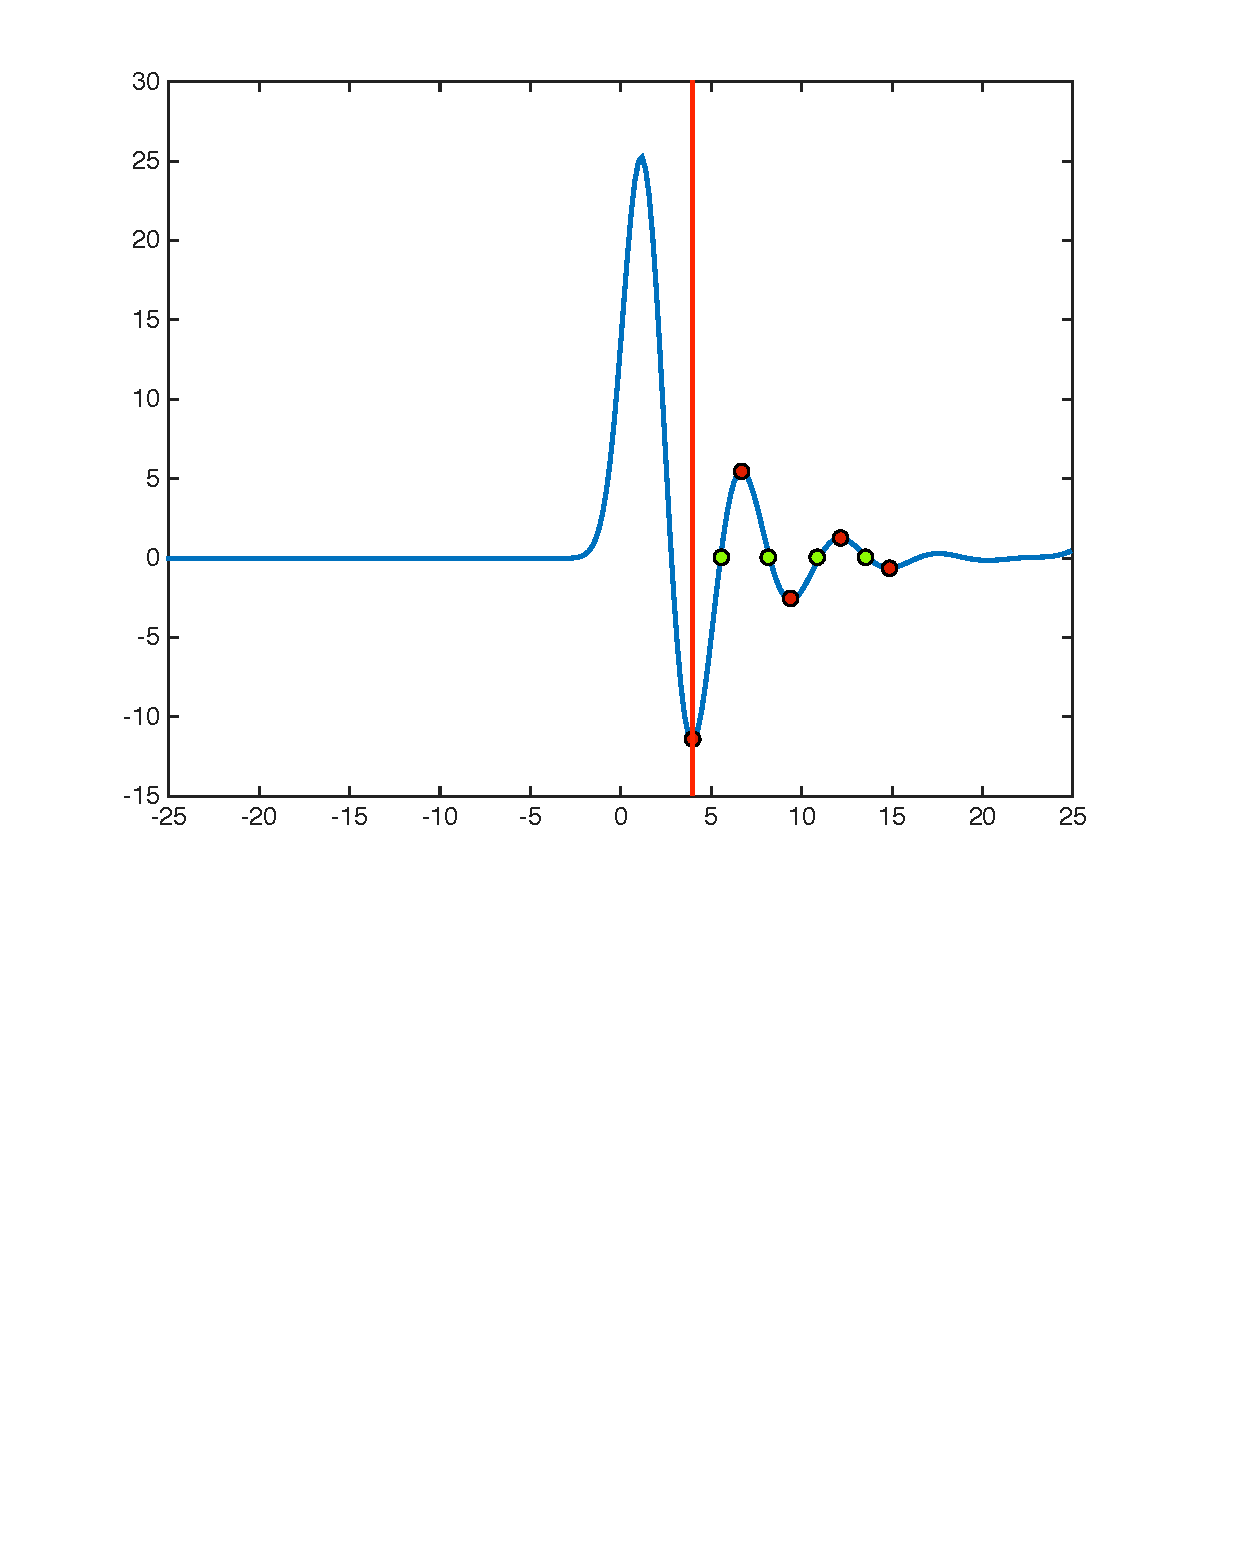
\includegraphics[width=0.8\linewidth]{images/singlepulsemagtailcut}
	\end{center}

\end{frame}

\begin{frame}
	\frametitle{Double Pulse Construction}
	1. Truncate
	\begin{center}
	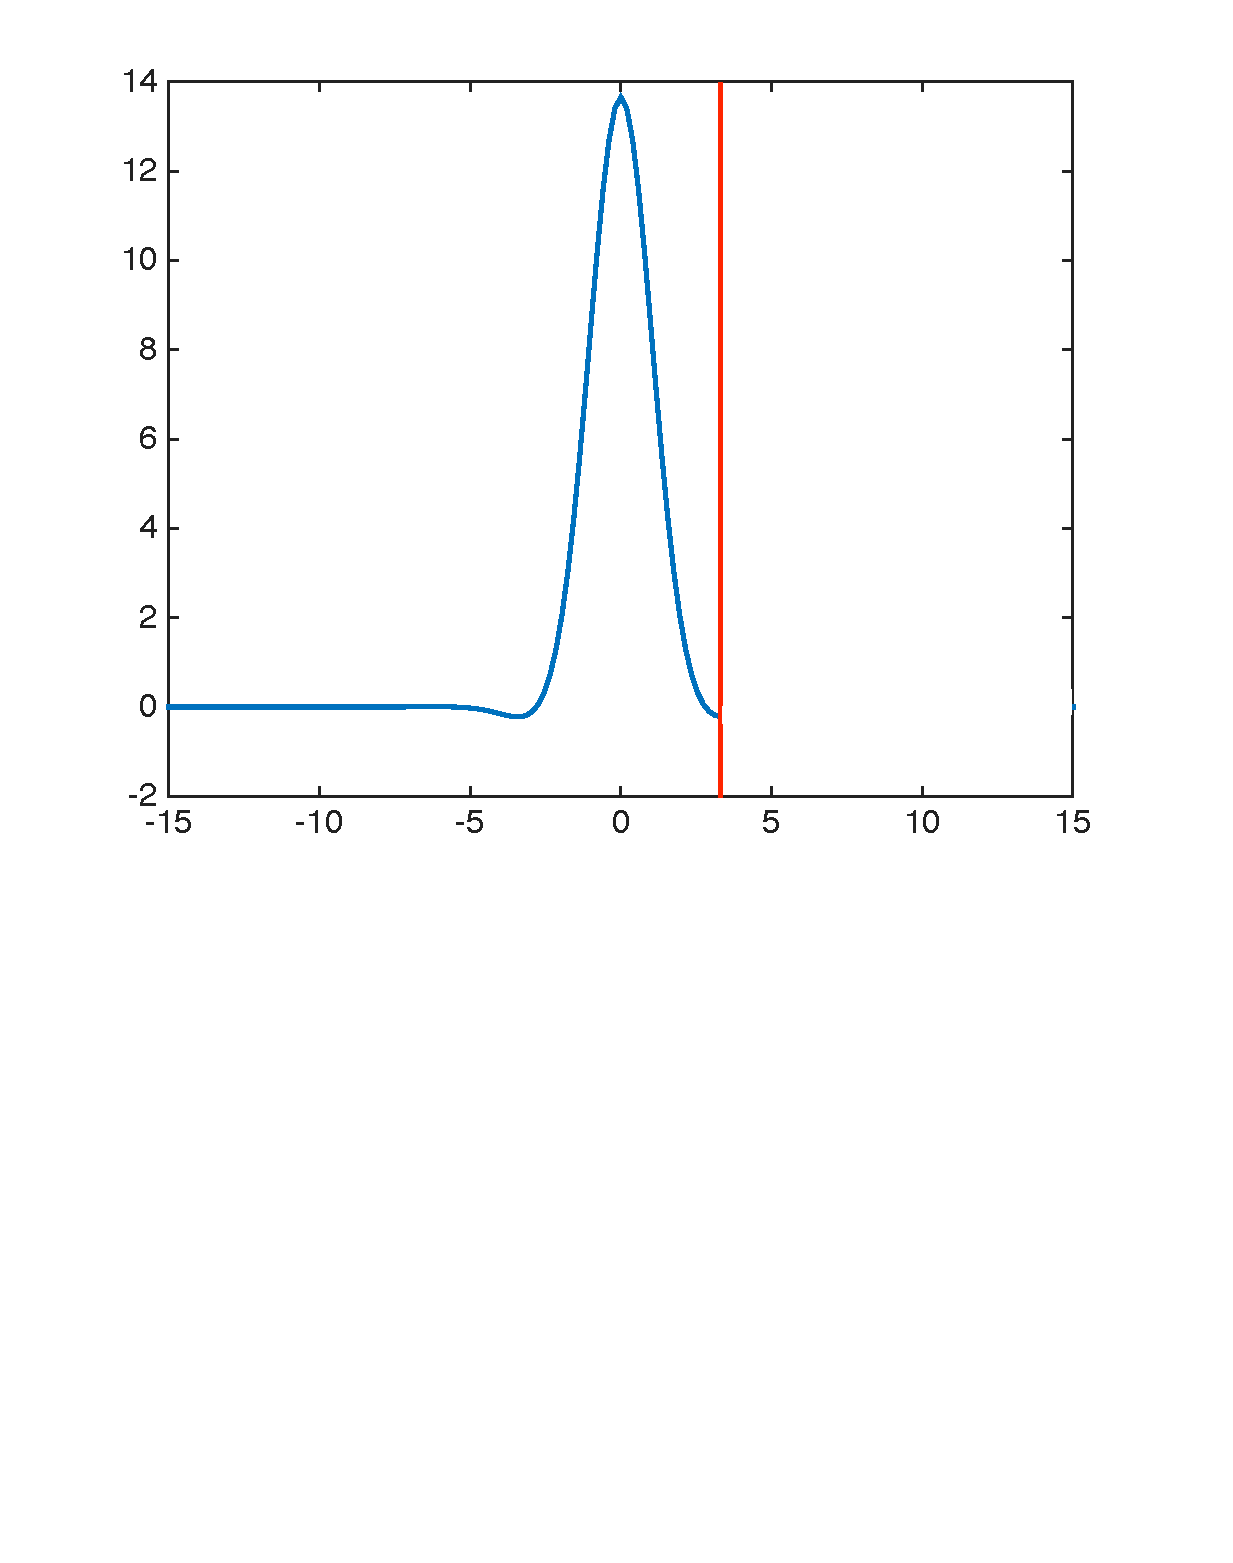
\includegraphics[width=0.8\linewidth]{images/single}
	\end{center}
\end{frame}

\begin{frame}
	\frametitle{Double Pulse Construction}
	1. Truncate
	\begin{center}
	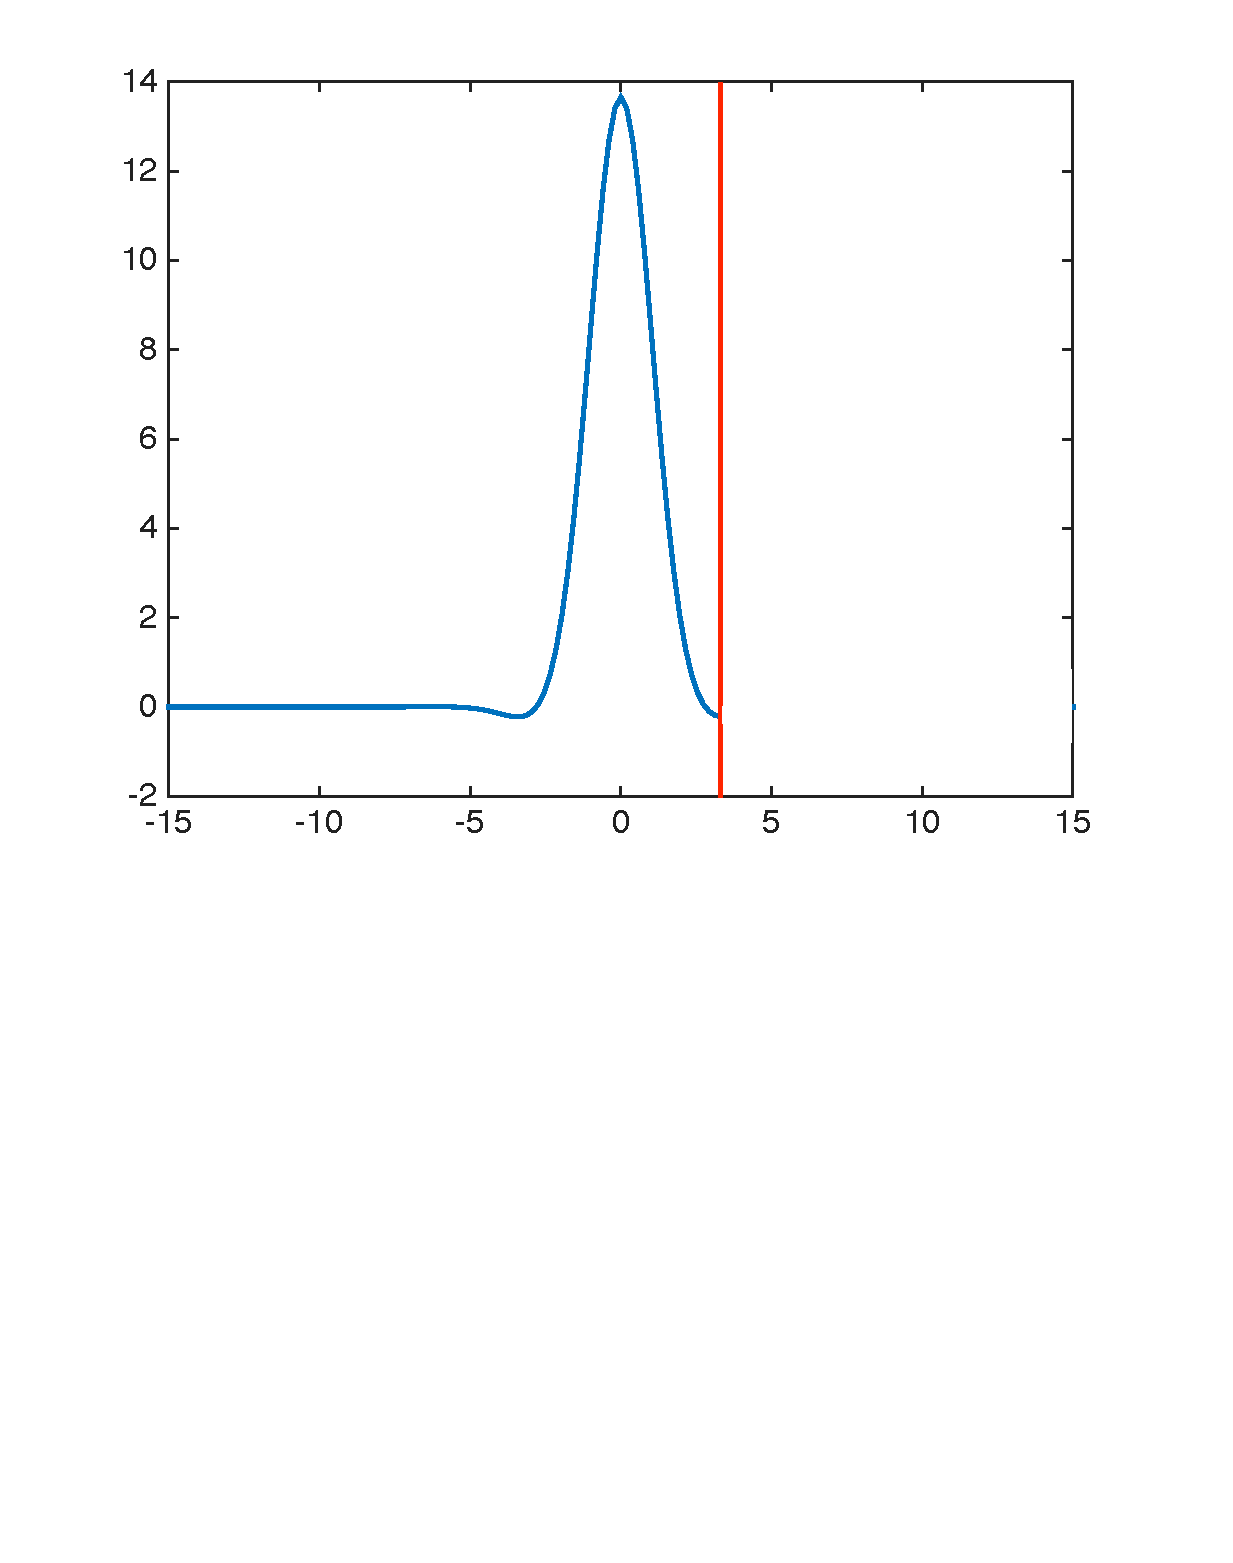
\includegraphics[width=0.8\linewidth]{images/singlecut}
	\end{center}
\end{frame}

\begin{frame}
	\frametitle{Double Pulse Construction}
	2. Mirror
	\begin{center}
	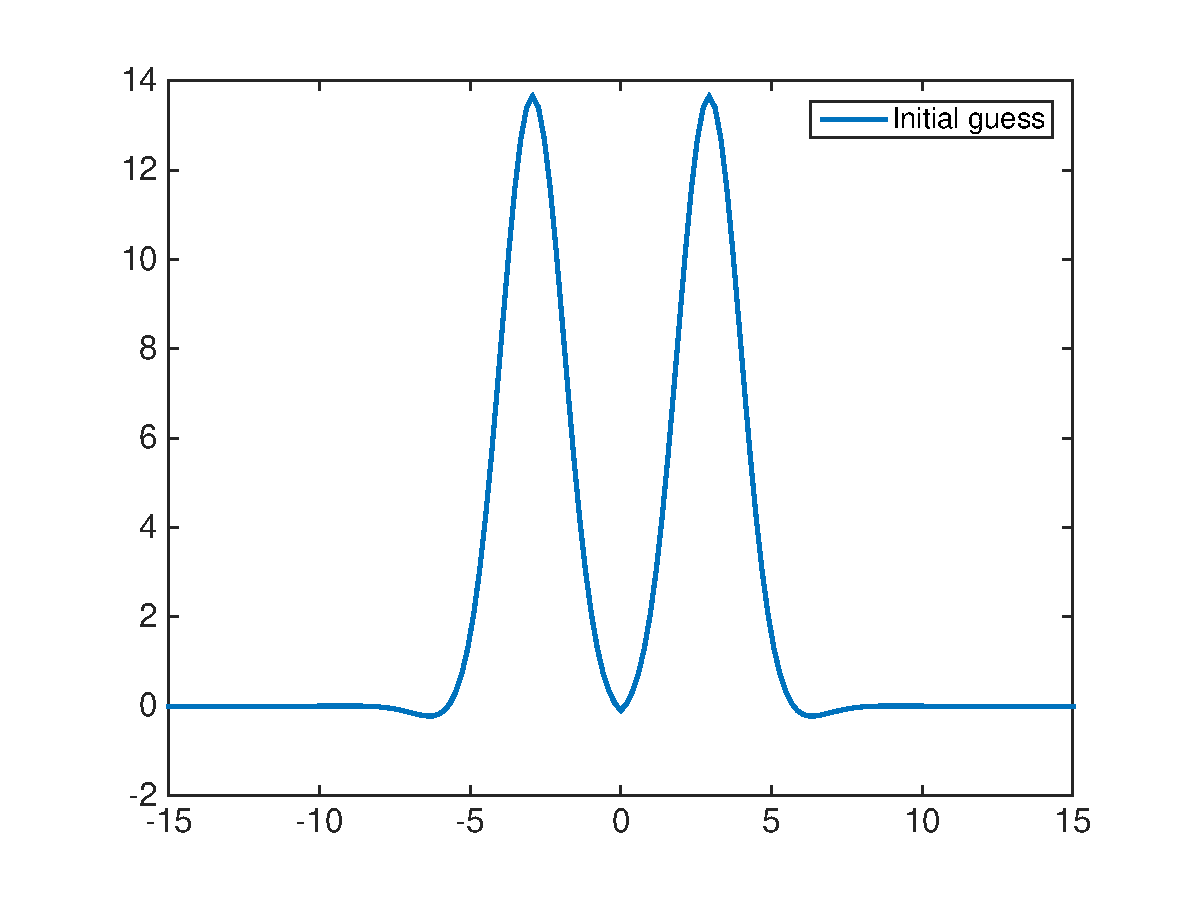
\includegraphics[width=0.8\linewidth]{images/dp1before.eps}
	\end{center}
\end{frame}

\begin{frame}
	\frametitle{Double Pulse Construction}
	3. Solve (numerically)
	\begin{center}
	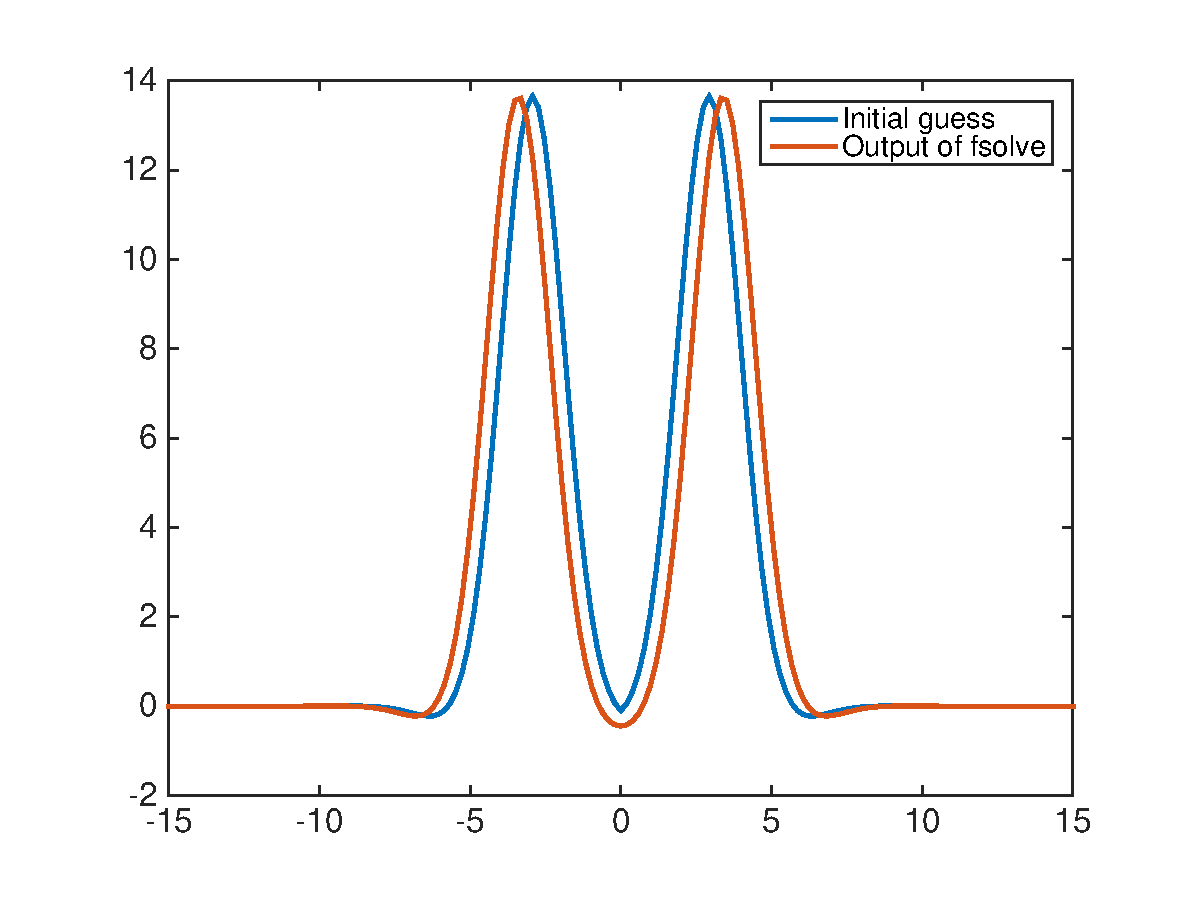
\includegraphics[width=0.8\linewidth]{images/dp1after.eps}
	\end{center}
\end{frame}

\begin{frame}
	\frametitle{Eigenvalues}
	\begin{itemize}
		\item Discretize eigenvalue problem $Lv = \lambda v$
		\item Compute eigenvalues of matrix $L$ with Matlab's \texttt{eig} function
		\item Similar results for Fourier and Chebyshev polynomial spectral methods
		\item We will show results for Fourier spectral methods
	\end{itemize}
\end{frame}

\begin{frame}
	\frametitle{Eigenvalues, unstable double pulse}
	\begin{figure}
   		\includegraphics[width=0.5\textwidth]{images/unstabledoublepulse}
   		\hfill
   		\includegraphics[width=0.5\textwidth]{images/unstabledoublepulse2}
	\end{figure}
\end{frame}

\begin{frame}
	\frametitle{Eigenvalues, unstable double pulse}
	\begin{figure}
   		\includegraphics[width=0.5\textwidth]{images/unstabledoublepulse}
   		\hfill
   		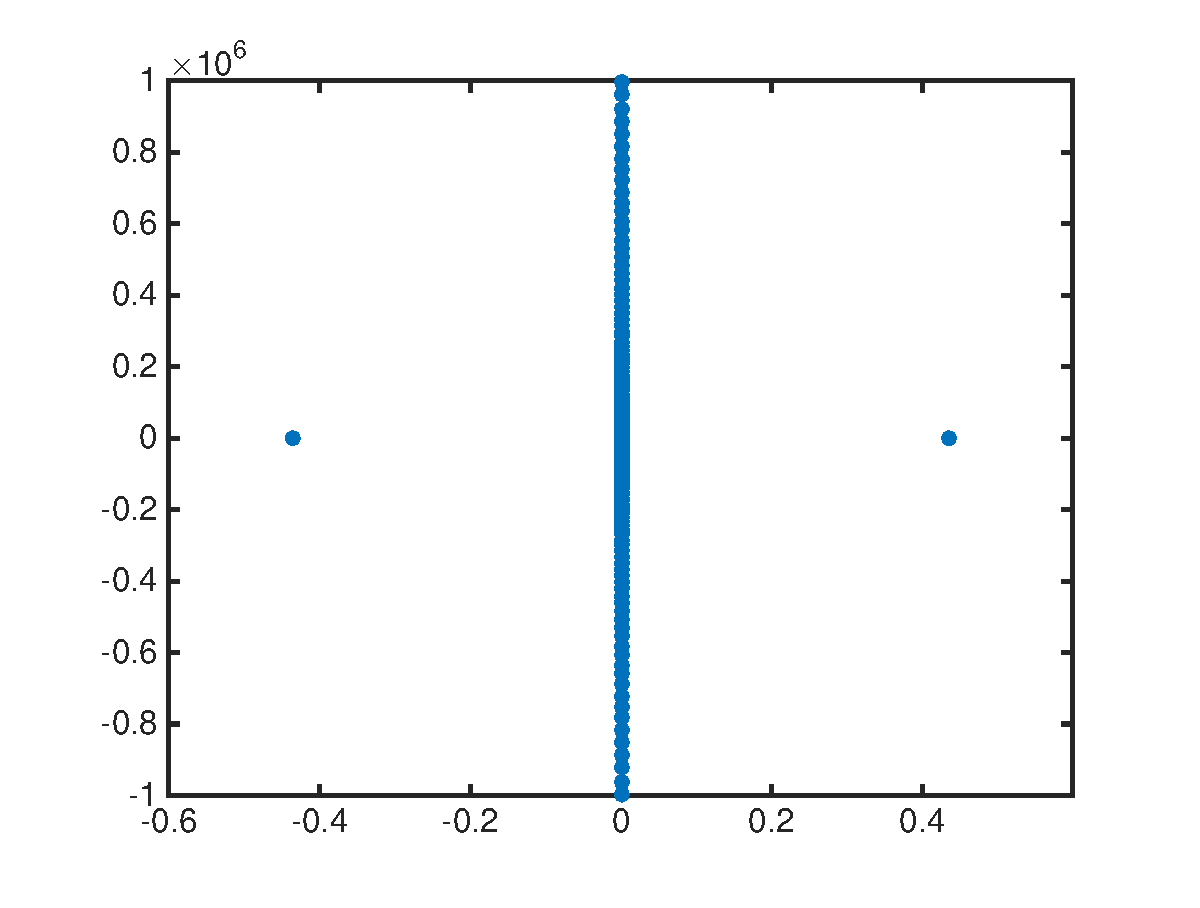
\includegraphics[width=0.5\textwidth]{images/unstableeig}
	\end{figure}
\end{frame}

\begin{frame}
	\frametitle{Eigenvalues, potentially stable double pulse}
	Potentially stable double pulse
	\begin{figure}
   		\includegraphics[width=0.5\textwidth]{images/stabledoublepulse}
   		\hfill
   		\includegraphics[width=0.5\textwidth]{images/stabledoublepulse2}
	\end{figure}
\end{frame}

\begin{frame}
	\frametitle{Eigenvalues, potentially stable double pulse}
	Potentially stable double pulse
	\begin{figure}
   		\includegraphics[width=0.5\textwidth]{images/stabledoublepulse}
   		\hfill
   		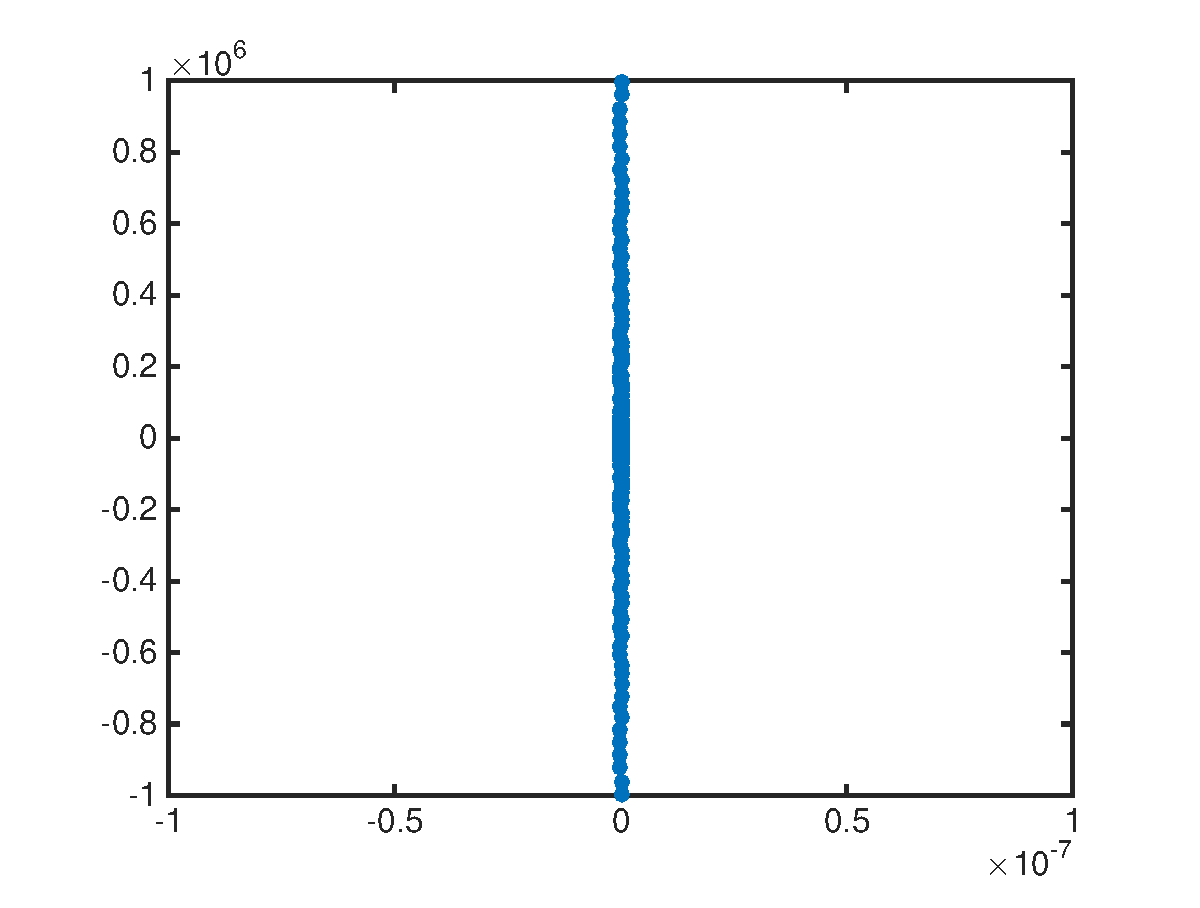
\includegraphics[width=0.5\textwidth]{images/stableeig}
	\end{figure}
\end{frame}

\begin{frame}
	\frametitle{Eigenvalues, weighted space}
	\begin{figure}
   		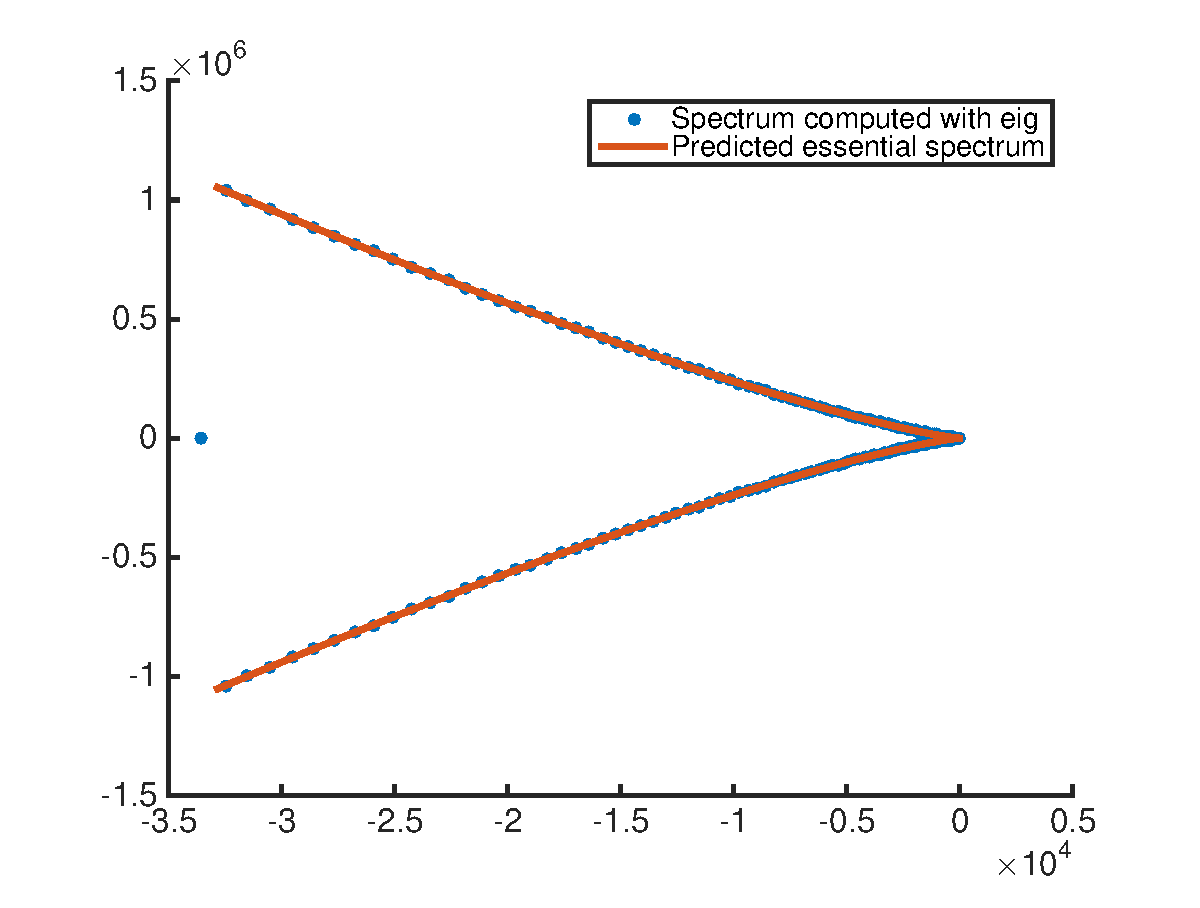
\includegraphics[width=0.5\textwidth]{images/stableeigweighted1}
   		\hfill
   		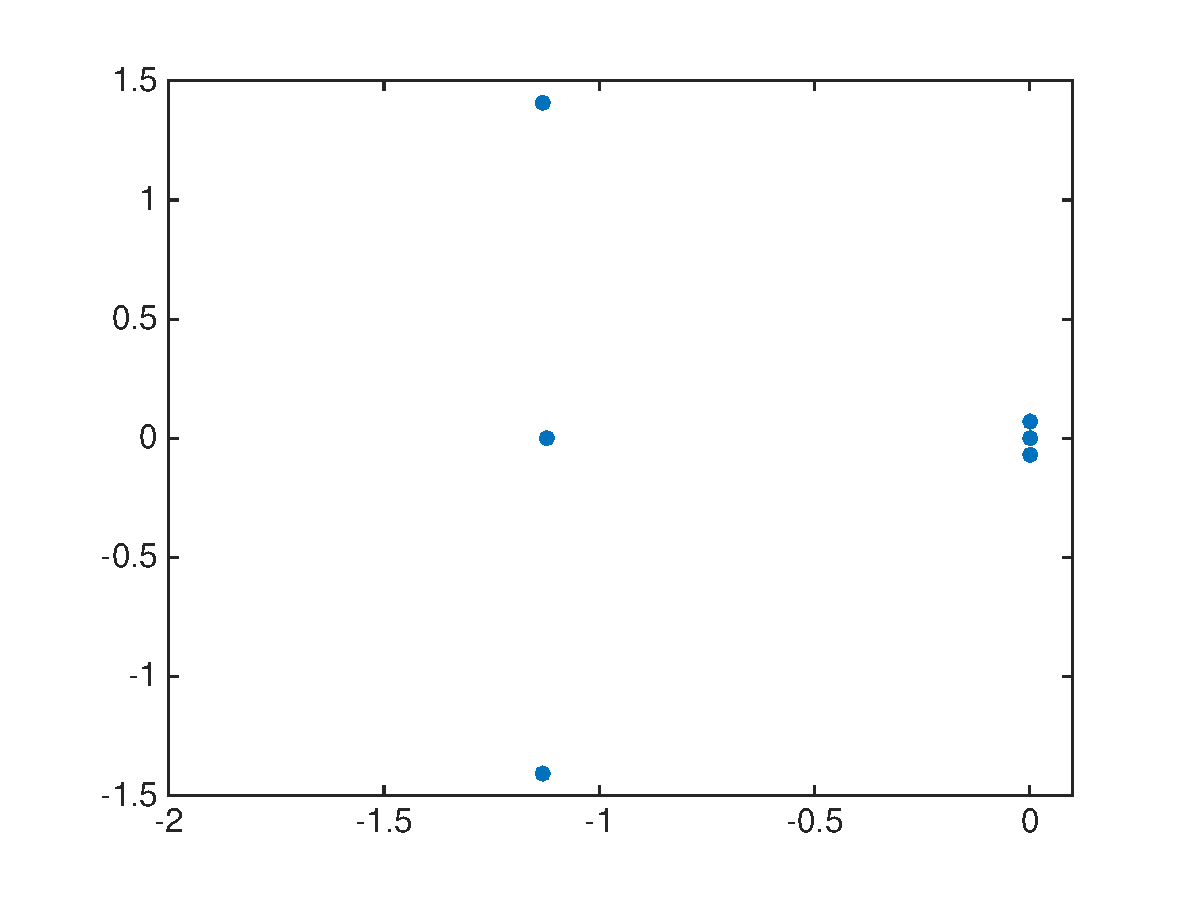
\includegraphics[width=0.5\textwidth]{images/stableeigweighted2}
	\end{figure}
\end{frame}

\begin{frame}
	\frametitle{Eigenvalues, unweighted space}

	\begin{block}{Nonzero point spectrum (interaction eigenvalues)}
		\[ \lambda = 2.0829 \times 10^{-11} \pm 0.0691i \]
	\end{block}
\end{frame}

\begin{frame}
	\frametitle{Eigenvalues, unweighted space}
	Is real part actually zero?
	\begin{itemize}
		\item<1->Real part of order $\times 10^{-11}$ suggests numerical error.
		\item<2->By symmetery of Hamiltonian system, would expect to see quadruplet of eigenvalues
		 \[ \lambda = \pm \: 2.0829 \times 10^{-11} \pm 0.0691i \]
		\item<3-> We can numerically construct a ``better'' eigenfunction $v$ with $\lambda$ pure imaginary such that $\max |Lv - \lambda v|$ is improved
		\item<4-> Krein matrix argument?
	\end{itemize}
\end{frame}

\begin{frame}
	\frametitle{Time stepping}
	\begin{itemize}
		\item<1->What really happens near the double-pulse equilibria?
		\item<2->Time-stepping scheme:
		\begin{itemize}
			\item Chebyshev polynomial spectral discretization in space
			\item Crank-Nicolson/Adams-Bashforth 2 IMEX scheme for time-stepping
		\end{itemize}
		\item<3->Initial condition: ``pull apart'' double pulses and let go!
	\end{itemize}
\end{frame}

\begin{frame}
	\frametitle{Time stepping, near unstable double pulse}
	\begin{center}
		\includemedia[
		     width=8cm,height=6cm,
		     activate=pageopen,
		     addresource=images/unstable.mp4,
		     flashvars={
		         source=images/unstable.mp4
		        &autoPlay=true
		     }
	]{}{VPlayer.swf} 
	\end{center}
\end{frame}

\begin{frame}
	\frametitle{Time stepping, near potentially stable double pulse}
	\begin{center}
		\includemedia[
		     width=8cm,height=6cm,
		     activate=pageopen,
		     addresource=images/stable.mp4,
		     flashvars={
		         source=images/stable.mp4
		        &autoPlay=true
		     }
	]{}{VPlayer.swf} 
	\end{center}
\end{frame}

\begin{frame}
	\frametitle{Phase portrait, near potentially stable double pulse}
	Plot distance between pulses vs. the derivative of this distance
	\begin{center}
	\includegraphics[width=0.6\linewidth]{images/phaseportrait1}
	\end{center}
\end{frame}

\begin{frame}
	\frametitle{Phase portrait}
	\begin{center}
	\includegraphics[width=0.8\linewidth]{images/phaseportrait2}
	\end{center}
\end{frame}

\begin{frame}
	\frametitle{Future directions}

\end{frame}

\begin{frame}
	\frametitle{References}
\end{frame}
 
\end{document}